\documentclass[11pt,a4paper]{article}
\usepackage[a4paper, margin=1.3in]{geometry}
\usepackage{mathtools}
\usepackage{fancyhdr}
\usepackage{mathrsfs}

\newcommand{\sheetNr}{9}

\pagestyle{fancy}
\fancyhf{}
\lhead{AI Planning}
\rhead{Exercise Sheet \sheetNr}
\lfoot{Axel Perschmann, Tarek Saier, \today}
\rfoot{Page \thepage\ of \pageref{lastpage}}
\renewcommand{\headrulewidth}{0.3pt}
\renewcommand{\footrulewidth}{0.3pt}
\setlength\parindent{0pt}
\newcommand{\h}[0]{\text{--}}

\begin{document}
\begin{center}
\Huge{\textbf{AI Planning}}\\
\LARGE{\textbf{Exercise Sheet \sheetNr}}
\end{center}
\vspace{2cm}
\begin{tabular}{ll}
Date: & \today\\
Students: & Axel Perschmann, Tarek Saier
\end{tabular}

\section*{Exercise 9.1}
\textbf{(a)} Compatibility graph:\\
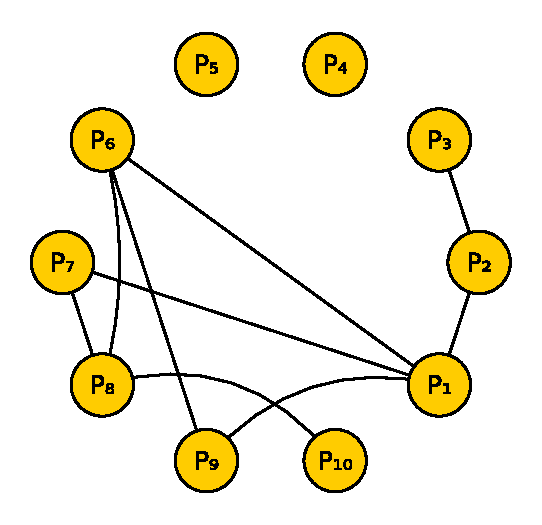
\includegraphics[scale=0.7]{compgraph}\\
Maximal cliques: $\{P_1,P_2\}$, $\{P_1,P_6,P_9\}$, $\{P_1,P_7\}$, $\{P_2,P_3\}$, $\{P_4\}$, $\{P_5\}$, $\{P_6,P_8\}$, $\{P_7,P_8\}$, $\{P_8,P_{10}\}$.\\
\\
\textbf{(b)}\\
$h^\mathscr{C}=max\{h^{P_1}+h^{P_2},h^{P_1}+h^{P_6}+h^{P_9},h^{P_1}+h^{P_7},h^{P_2}+h^{P_3},h^{P_4},h^{P_5},h^{P_6}+h^{P_8},h^{P_7}$\\
\hphantom{tabta}$+h^{P_8},h^{P_8}+h^{P_{10}}\}$\\
\hphantom{tab}$=max\{h^{\{at\h goal_{s2}\}}+h^{\{at\h goal_{s1},position_{s1}\}},h^{\{at\h goal_{s2}\}}+h^{\{at\h goal_{s1},content_H\}}+$\\
\hphantom{tabta}$h^{\{content_A,content_E\}},h^{\{at\h goal_{s2}\}}+h^{\{at\h goal_{s1},content_G\}},h^{\{at\h goal_{s1},position_{s1}\}}+$\\
\hphantom{tabta}$h^{\{at\h goal_{s2},position_{s2}\}},h^{\{at\h goal_{s1},position_{s1},position_{p}\}},h^{\{position_{s1},position_{p}\}},$\\
\hphantom{tabta}$h^{\{at\h goal_{s1},content_H\}}+h^{\{at\h goal_{s2},content_D\}},h^{\{at\h goal_{s1},content_G\}}+h^{\{at\h goal_{s2},content_D\}},$\\
\hphantom{tabta}$h^{\{at\h goal_{s2},content_D\}}+h^{\{at\h goal_{s1},content_Q\}}\}$\\
\\
Algebraic implification:\\
$h^\mathscr{C}=max\{h^{\{at\h goal_{s2}\}}+max\{h^{\{at\h goal_{s1},position_{s1}\}},h^{\{at\h goal_{s1},content_H\}}+h^{\{content_A,content_E\}},$\\
\hphantom{tabta}$h^{\{at\h goal_{s1},content_G\}}\},h^{\{at\h goal_{s1},position_{s1}\}}+h^{\{at\h goal_{s2},position_{s2}\}},h^{\{at\h goal_{s1},position_{s1},position_{p}\}},$\\
\hphantom{tabta}$h^{\{position_{s1},position_{p}\}},h^{\{at\h goal_{s2},content_D\}}+max\{h^{\{at\h goal_{s1},content_H\}},h^{\{at\h goal_{s1},content_G\}},$\\
\hphantom{tabta}$h^{\{at\h goal_{s1},content_Q\}}\}\}$\\
Dominance pruning:\\
$h^\mathscr{C}=max\{h^{\{at\h goal_{s2}\}}+max\{h^{\{at\h goal_{s1},position_{s1}\}},h^{\{at\h goal_{s1},content_H\}}+h^{\{content_A,content_E\}},$\\
\hphantom{tabta}$h^{\{at\h goal_{s1},content_G\}}\},h^{\{at\h goal_{s1},position_{s1}\}}+h^{\{at\h goal_{s2},position_{s2}\}},h^{\{at\h goal_{s1},position_{s1},position_{p}\}},$\\
\hphantom{tabta}$h^{\{at\h goal_{s2},content_D\}}+max\{h^{\{at\h goal_{s1},content_H\}},h^{\{at\h goal_{s1},content_G\}},h^{\{at\h goal_{s1},content_Q\}}\}\}$\newpage
\textbf{(c)} Obviously not reasonable is:\\
\begin{tabular}{c|l}
Pattern & Reason\\
\hline
$P_9$ & random positions, no relevance for goal\\
\end{tabular}\\
\\
Most likely not reasonable are:\\
\begin{tabular}{c|l}
Pattern & Reason\\
\hline
$P_{6-8,10}$ & one goal relevant variable + random position\\
$P_1$ & by itself reasonable, but included in $P_3$\\
$P_5$ & by itself reasonable, but included in $P_4$\\
\end{tabular}\\
\\
$h^\mathscr{C}=max\{h^{P_2}+h^{P_3},h^{P_4}\}$\\

\section*{Exercise 9.2}
Variables being connected in the CG means that they are relevant for modifying each other. If we start with $P$ such that \emph{all} its variables are causally relevant and $P$ is causally connected and further pick $v$ such that $P'$ is \emph{still} causally connected, then $v$ cannot have been an intermediate node in the CG. It can only be the case that $v$ in the CG was either (1) pointing at some variable still present in $P'$ or (2) being pointed at by some variable still present in $P'$ and pointing at $\gamma$.

\label{lastpage}
\end{document}
